\documentclass[tikz,border=2pt,11pt]{standalone}
\usepackage{amsmath}
\usepackage{amssymb}
\usepackage{xcolor}
\usepackage{tikz}
\newcommand{\Clust}{\operatorname{Clust}}
\newcommand{\val}{\operatorname{val}}
\newcommand{\OBJ}{\operatorname{OBJ}}
\newcommand{\Inf}{\operatorname{Inf}}
\newcommand{\one}{\mathbf 1}
\newcommand{\E}{\mathbb E}
\newcommand{\R}{\mathbb R}
\newcommand{\Q}{\mathbb Q}
\newcommand{\N}{\mathbb N}
\begin{document}
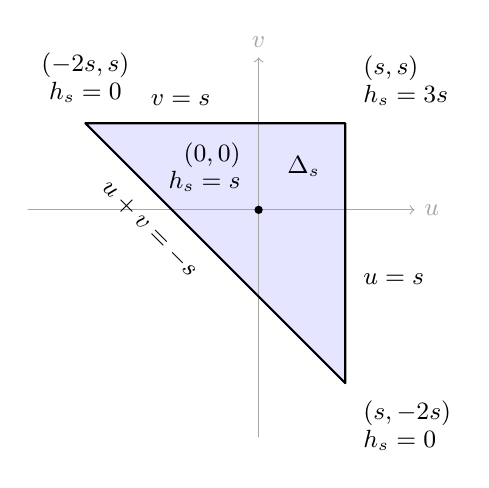
\begin{tikzpicture}[x=1.10cm,y=1.10cm,line cap=round,line join=round,
                      font=\small]
    \fill[blue!10] (-2,1) -- (1,1) -- (1,-2) -- cycle;
    \draw[gray!70,->] (-2.66,0) -- (1.80,0) node[right] {$u$};
    \draw[gray!70,->] (0,-2.62) -- (0,1.76) node[above] {$v$};
    \draw[thick] (-2,1) -- (1,1) -- (1,-2) -- cycle;
    \node[above=4pt,align=center] at (-2,1)
      {$(-2s,s)$\\[-1pt] $h_s=0$};
    \node[above right=3pt,align=left] at (1,1)
      {$(s,s)$\\[-1pt] $h_s=3s$};
    \node[below right=3pt,align=left] at (1,-2)
      {$(s,-2s)$\\[-1pt] $h_s=0$};
    \node[above=3pt] at (-.90,1) {$v=s$};
    \node[right=3pt] at (1,-.80) {$u=s$};
    \node[rotate=-45,below=4pt] at (-1.02,.02) {$u+v=-s$};
    \node at (.52,.50) {$\Delta_s$};
    \fill (0,0) circle[radius=1.5pt];
    \node[above left=3pt,align=right] at (0,0)
      {$(0,0)$\\[-1pt] $h_s=s$};
  \end{tikzpicture}
\end{document}
